% Copyright 2020 by Tara Prasad Mishra <tara.13.1996@gmail.com>.
%
% This is a template adapted from Wang Kunzhen's Beamer template for 
% Singapore-MIT Alliance (LEES IRG Users).
% In principle, this file can be redistributed and/or modified under
% the terms of the GNU Public License, version 2.
%
% However, this file is supposed to be a template to be modified
% for your own needs. For this reason, if you use this file as a
% template and not specifically distribute it as part of a another
% package/program, I grant the extra permission to freely copy and
% modify this file as you see fit and even to delete this copyright
% notice. 

\documentclass[xcolor=dvipsnames]{beamer}
\usepackage{transparent}
% There are many different themes available for Beamer. A comprehensive
% list with examples is given here:
% http://deic.uab.es/~iblanes/beamer_gallery/index_by_theme.html
% You can uncomment the themes below if you would like to use a different
% one:
%\usetheme{AnnArbor}
%\usetheme{Antibes}
%\usetheme{Bergen}
% \usetheme{Berkeley}
%\usetheme{Berlin}
%\usetheme{Boadilla}
% \usetheme{boxes}
%\usetheme{CambridgeUS}
\usetheme{Copenhagen}
%\usetheme{Darmstadt}
%\usetheme{default}
%\usetheme{Frankfurt}
%\usetheme{Goettingen}
%\usetheme{Hannover}
% \usetheme{Ilmenau}
% \usetheme{JuanLesPins}
% \usetheme{Luebeck}
% \usetheme{Madrid}
%\usetheme{Malmoe}
%\usetheme{Marburg}
% \usetheme{Montpellier}
% \usetheme{PaloAlto}
% \usetheme{Pittsburgh}
% \usetheme{Rochester}
% \usetheme{Singapore}
% \usetheme{Szeged}
% \usetheme{Warsaw}

\definecolor{nus-orange}{RGB}{239,124,0} 
\definecolor{nus-white}{RGB}{255,255,255}
\definecolor{nus-blue}{RGB}{0,61,124}
\definecolor{nus-black}{RGB}{0,0,0}

% Uncomment this section if you want the title background for each slide to be gradient like decaying from nus-orange to nus-white.
% \useoutertheme{shadow}
% \usepackage{tikz}
% \usetikzlibrary{shadings}
% \colorlet{titleleft}{nus-orange}
% \colorlet{titleright}{nus-orange!45!nus-white}
% \makeatletter
% \pgfdeclarehorizontalshading[titleleft,titleright]{beamer@frametitleshade}{\paperheight}{%
%   color(0pt)=(titleleft);
%   color(\paperwidth)=(titleright)}
% \makeatother
% End of gradient slide title effect.

\setbeamercolor{section in head/foot}{bg=nus-blue, fg=nus-white}
\setbeamercolor{subsection in head/foot}{bg=nus-blue, fg=nus-white}
\setbeamercolor{frametitle}{bg=nus-orange, fg=nus-black}
\setbeamercolor{title}{bg=nus-orange, fg=nus-white}
\setbeamercolor{alerted text}{fg=nus-orange}
\setbeamercolor{block title}{fg=nus-blue}
\setbeamercolor{block body}{fg=nus-black}

\setbeamertemplate{theorems}[numbered]
\setbeamertemplate{propositions}[numbered]

\setbeamertemplate{bibliography item}{\insertbiblabel}

\setbeamertemplate{title page}[default][colsep=-4bp,rounded=true, shadow=true]

\title{Title of the presentation}

\subtitle{Sub-title}

\author{Authors' names}

\institute[Singapore-MIT Alliance for Research and Technology] % (optional, but mostly needed)
{
  Low Energy Electronic System\\
  Singapore-MIT Alliance for Research and Technology
}

\titlegraphic{
   
\includegraphics[width=2cm]{smart-logo}
}

\date{03 Jan 2020}

% Uncomment this, if you want the table of contents to pop up at
% the beginning of each subsection:
% \AtBeginSubsection[]
% {
%   \begin{frame}<beamer>{Outline}
%     \tableofcontents[currentsection,currentsubsection]
%   \end{frame}
% }



\begin{document}
{
\setbeamertemplate{background}
{\transparent{0.2}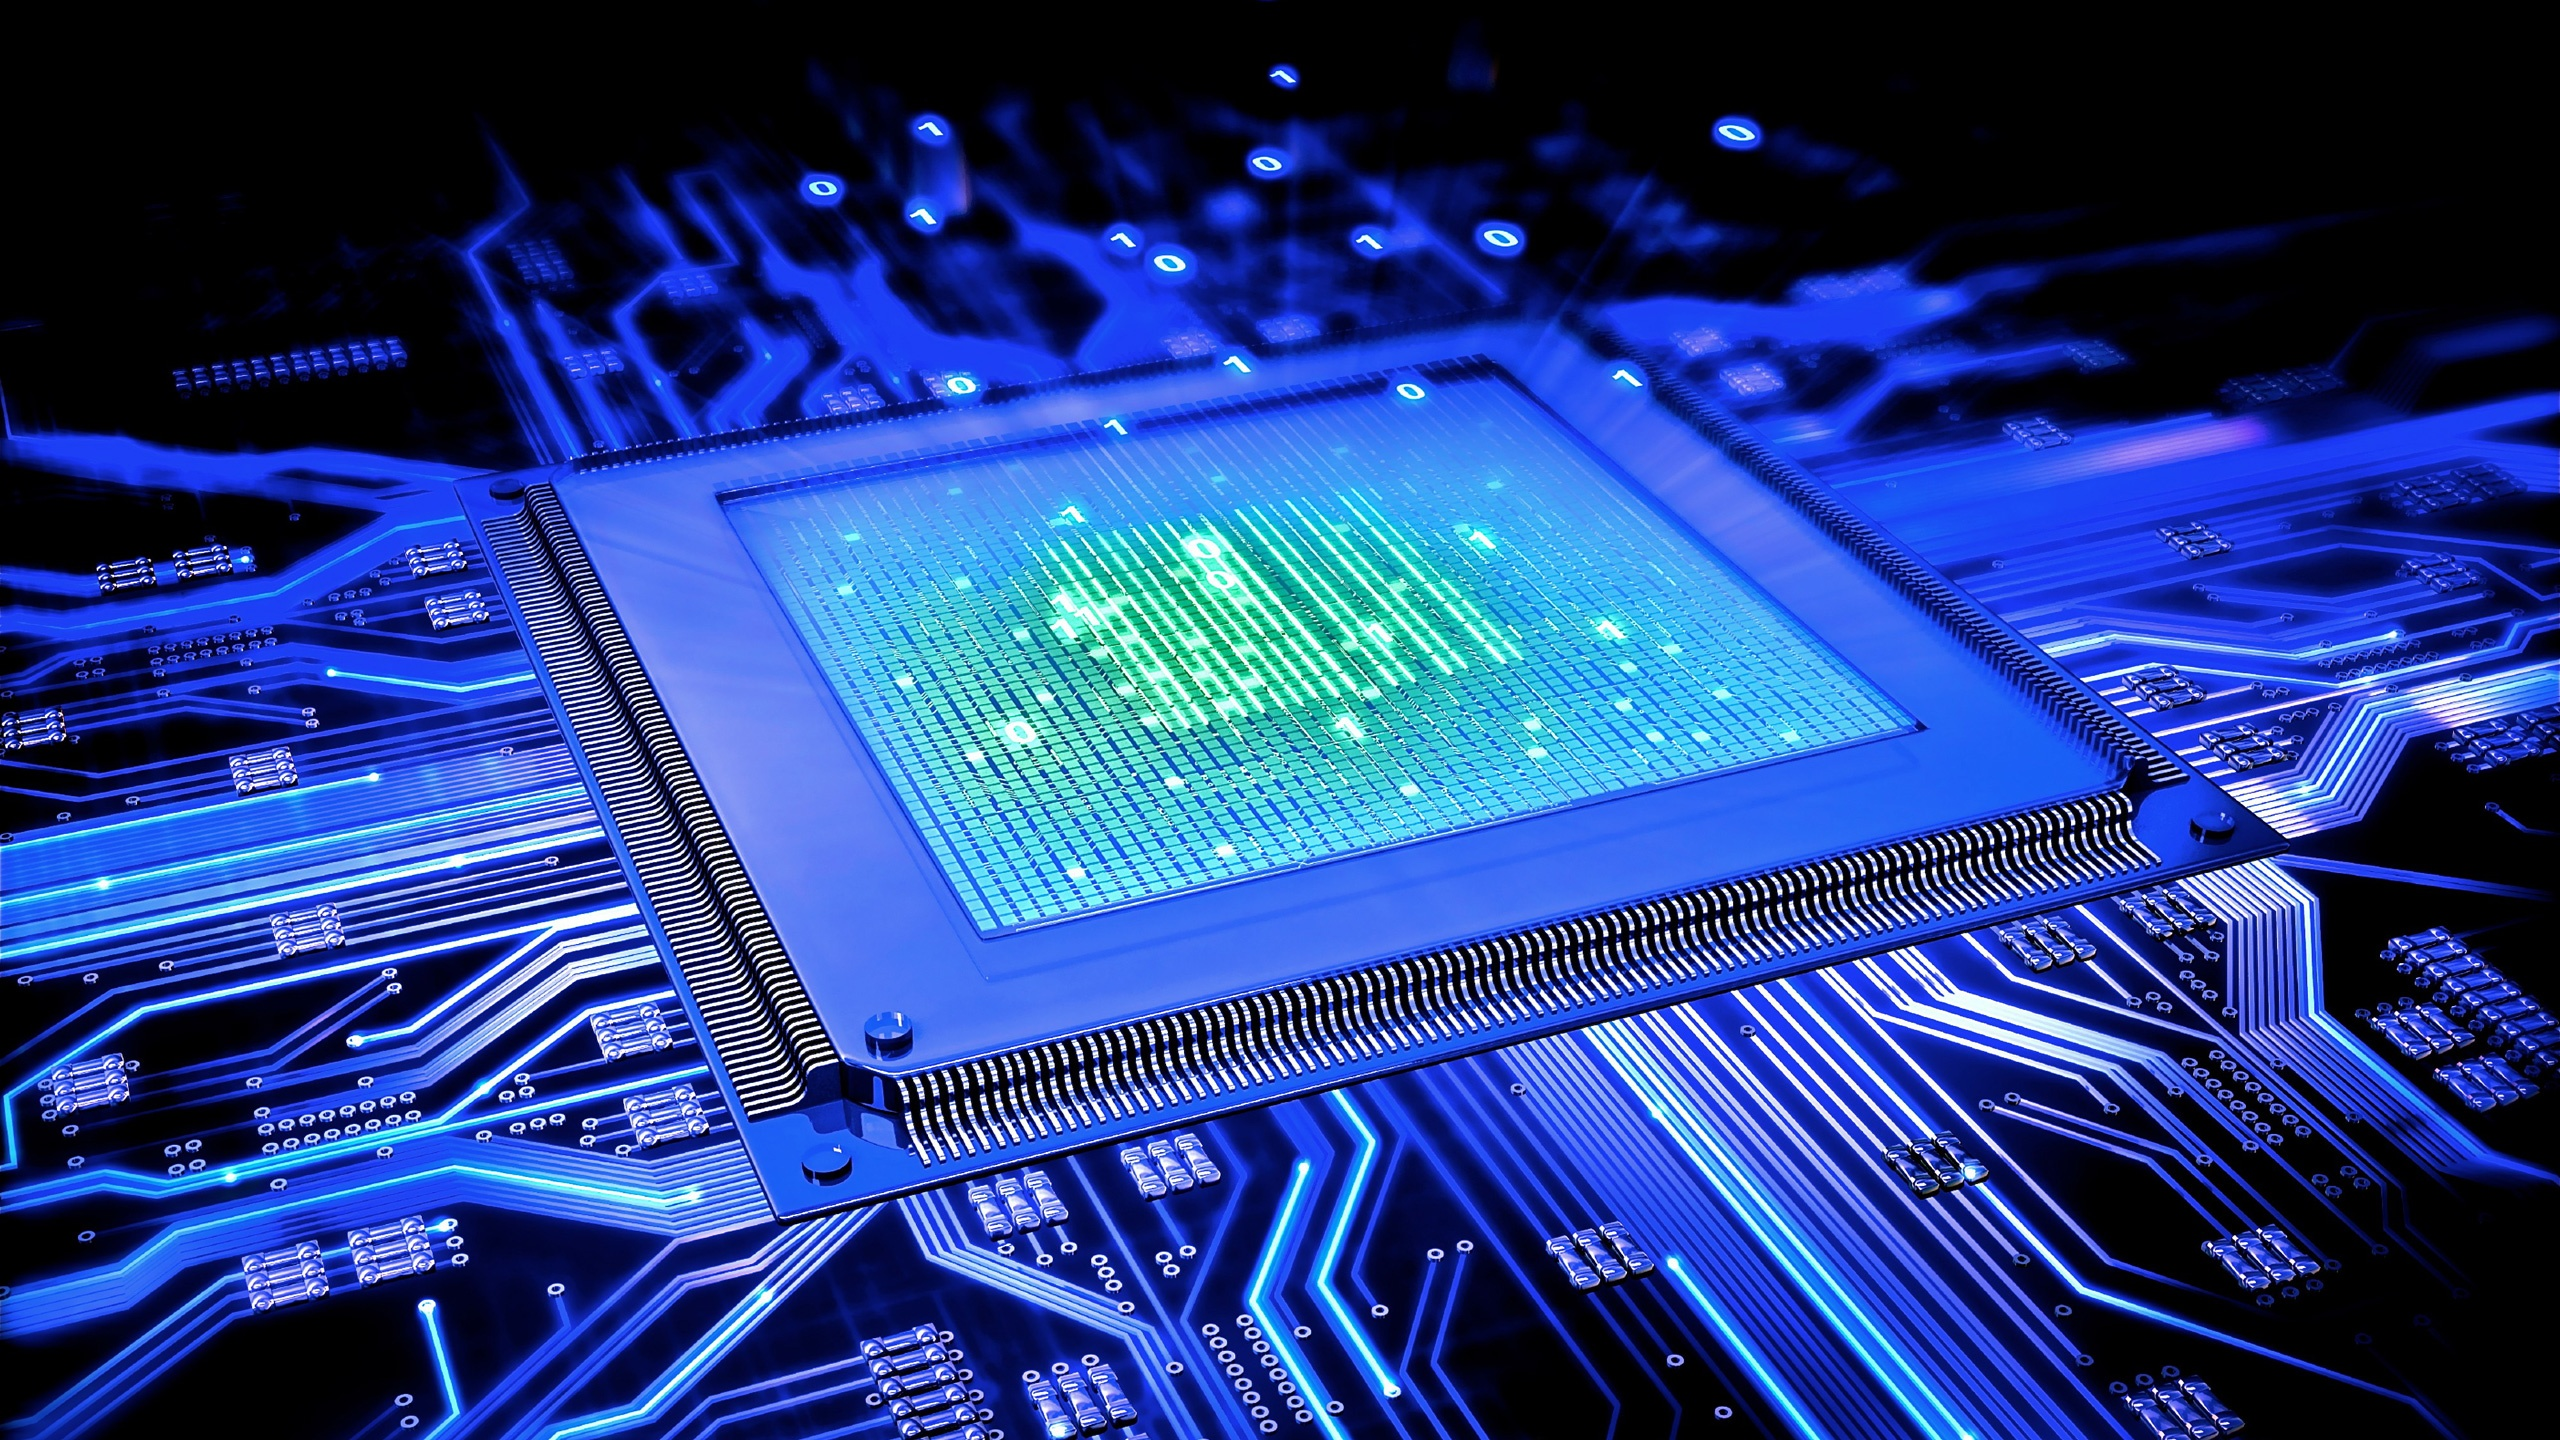
\includegraphics[width=\paperwidth,height=\paperheight]{firstpage.jpeg}}
\setbeamercolor{normal text}{fg=black}\usebeamercolor*{normal text}
\begin{frame}
  \titlepage
\end{frame}
}

\begin{frame}{Outline}
  \tableofcontents
\end{frame}

\section{First Main Section}

\subsection{First Subsection}
\begin{frame}{First Slide Title}{Optional Subtitle}
  \begin{itemize}
  \item {
    My first point.
  }
  \item {
    My second point.
  }
  \end{itemize}
\end{frame}

\subsection{Second Subsection}
% You can reveal the parts of a slide one at a time
% with the \pause command:
\begin{frame}{Second Slide Title}
  \begin{itemize}
  \item {
    First item.
    \pause % The slide will pause after showing the first item
  }
  % You can also specify when the content should appear
  % by using <n->:
  \item<3-> {
    Third item.
  }
  % or you can use the \uncover command to reveal general
  % content (not just \items):
  \item<5-> {
    Fifth item. \uncover<6->{Extra text in the fifth item.}
  }
  \end{itemize}
\end{frame}

\section{Second Main Section}

\subsection{Second Subsection}
\begin{frame}{Main Theorem}
\begin{theorem}
Theorem Statements. Example for citation \cite{Author1990}.
\end{theorem}

\begin{proof}
Proof of the theorem goes here.
\end{proof}
\end{frame}

% Placing a * after \section means it will not show in the
% outline or table of contents.
\section*{Summary}

\begin{frame}{Summary}
  \begin{itemize}
  \item
    The \alert{first main message} of your talk in one or two lines.
  \item
    The \alert{second main message} of your talk in one or two lines.
  \item
    Perhaps a \alert{third message}, but not more than that.
  \end{itemize}
  
  \begin{itemize}
  \item
    Outlook
    \begin{itemize}
    \item
      Something you haven't solved.
    \item
      Something else you haven't solved.
    \end{itemize}
  \end{itemize}
\end{frame}

% Bibliography section. Use \bibitem to add more bibliography items.
\section*{Bibliography}
\begin{frame}{Bibliography}
  \begin{thebibliography}{10}

  \bibitem{Author1990}
    A.~Author.
    \newblock {\em Handbook of Everything}.
    \newblock Some Press, 1990.

  \bibitem{Someone2000}
    S.~Someone.
    \newblock On this and that.
    \newblock {\em Journal of This and That}, 2(1):50--100,
    2000.

  \end{thebibliography}
\end{frame}

\end{document}